
%\newcommand{\MLP}{\text{MLP}}
%\newcommand{\FeedForward}{\text{FeedForward}}
%\newcommand{\Softmax}{\text{Softmax}}
%\newcommand{\reals}{\mathbb{R}}
\def\m{m}


\section{The Abstractor Framework}
\label{sec:abstractor_framework}

At a high level, the primary function of an abstractor is to compute abstract relational features of its
inputs\footnote{In this paper, we will tend to use the name `Abstractor' to refer to both the module, the framework, and models which contain the Abstractor module as a main component.}. That is, given a set of input objects $o_1, \ldots, o_\m$, the relational abstractor learns to model a relation $r(\cdot, \cdot)$ and computes a function on
the set of pairwise relations between objects ${\{ r(o_i, o_j) \}}_{ij}$. The relations and the computations on them are learned to carry out a specific prediction task (often end-to-end, but, crucially, the Abstractor framework naturally supports modular learning).
\subsection{Relational symbolic message-passing}
\label{ssec:message_passing}

At the core of abstractors is an operation we refer to as \textit{relational symbolic message-passing}.
The input to this operation is a relation tensor $R = \left[r(o_i, o_j)\right]_{i,j=1}^\m$, where $r(o_i, o_j) \in \mathbb{R}^{d_r}$ is a vector describing the relation between object $o_i$ and object $o_j$. We will come back to how an abstractor models pairwise relations and computes the relation tensor in the next subsection.

The starting point of symbolic message-passing is a set of learnable symbols $s_1, \ldots, s_\m \in \mathbb{R}^{d_s}$, where the hyperparameter $d_s$ is the dimension of the symbolic vectors. We call these parameters \textit{symbols} because each of them references (or ``is bound to") a particular object, but they are independent of the values of these objects. That is, the $i$th symbol references the $i$th object, but the value of $s_i$ is independent of the value of $o_i$. The use of those learned input-indpendent symbols is how symbolic message-passing achieves its abstraction.

In relational symbolic message-passing, we perform message-passing on these learned symbolic parameters according to the relation tensor $R$. In general, this message-passing operation can be described as a set-valued function of the form
\begin{equation}
    \label{eq:symbolic_message_passing}
    s_i \leftarrow \text{Update}\Big( s_i, \ \left\{ \left(R[i,j], s_j\right)\right\}_{j\in[m]}\Big), \quad i = 1, \ldots, m
\end{equation}
That is, the value of the $i$th symbol is updated as a function of the set of tuples $(R[i,j], s_j)$ of the relations with all other objects and the symbols of these objects. The symbols $s_j$ are naturally viewed
as values on the nodes of a graph, and the relations $R[i,j]$ are naturally viewed as weights on the edges. A simple but important special case of this is
\begin{equation}
    \label{eq:linear_symbolic_mp}
    s_i \leftarrow \sum_{j=1}^{m} R[i,j] s_j, \quad i=1, \ldots, m
\end{equation}
In the above, suppose that $d_r = 1$. Otherwise, the above operation is done for each dimension of the relation $R$ and the result is concatenated (similar to multi-head attention).

Following message-passing, each updated symbol $s_i$, can be passed through a feedforward neural network $f:\reals^{d_s}\rightarrow \reals^{d_s}$ to compute a non-linear function of the output. %Empirically, a residual connection and layer normalization may be useful, as in a transformer.
This message-passing operation can be repeated multiple times to iteratively update the symbolic vectors.  The output of relational symbolic message-passing is the set of abstracted symbols $A$ at the end of this sequence of message-passing operations. %The overall procedure is summarized in Algorithm~\ref{alg:relational_abstractor}.
In Section~\ref{sec:function_spaces} we characterize the class of functions on relations that this operation can compute.

% JDC: Shouldn't $d_s$ be included in the list of hyperparameters below?
%\begin{algorithm}[th!]
%    \caption{Relational Abstractor}\label{alg:relational_abstractor}
%    \SetKwFor{For}{for}{do}{end}
%    \SetKwInOut{Input}{Input}
%    \SetKwInOut{Output}{Output}
%    \SetKwInOut{LearnableParams}{Learnable parameters{\ }}
%    \SetKwInOut{HyperParams}{Hyperparameters}
%
%    \Input{Encoder entities: $E = (o_1, \ldots, o_\m) \in \mathbb{R}^{d_e \times m}$}
%    \HyperParams{$L$ (number of layers), $H$ (number of heads), feedforward network structure}
%    \LearnableParams{Symbols $S \in \reals^{d_s \times m}$, parameters $\{\theta_l\}$ of attention heads and feedforward models}
%    \Output{Abstracted sequence: $A = (a_1, \ldots, a_\m) \in \reals^{d_a \times m}$}
%    \vspace{1em}
%
%    $A \gets S$
%
%    \For{$l \gets 1$ \KwTo $L$}{
%        $A \gets \text{SelfAttention}_{\theta_l}(A)$\;
%        $A \gets \crossattend{E}{E}{A}{\theta_l}$\;
%        $A \gets\FeedForward_{\theta_l}(A)$\;
%        }
%\end{algorithm}
%
%\subsection{Computing the relation tensor with relational cross-attention}
%
%Symbolic message passing is the first of the two main
%%ingredients
%components
%of abstractors. What remains is to describe how the abstractor computes the relation tensor $R$. This is
%done through a variant of transformer cross-attention that we refer to as \textit{relational cross-attention}.
%To motivate this, we first describe how we can compute relations between pairs of objects through inner products.
%The inner product operation is a natural way to capture notions of relations and similarity. In Euclidean space,
%inner products capture the geometric alignment between vectors. Similarly, for objects with vector representations,
%inner products between these vector representations can capture relations between these objects.
%
%In general, we can formulate inner product relations as the standard Euclidean inner product between a pair of transformed object vectors. That is, 
%\begin{equation}
%    R(o_i, o_j) = \langle \phi(o_i), \psi(o_j) \rangle
%    \label{eq:relation_innerproduct}
%\end{equation}
%This captures a large class of relation functions. In particular, the theory of reproducing kernel Hilbert spaces implies that any continuous, symmetric function on pairs of objects can be approximated with such functions
%\citep{universal}. Multi-dimensional relation functions can be achieved by stacking multiple such inner products.
%In the next section we frame this explicitly in terms of transformer operations.
%
%% NOTE / TODO: need to describe what we mean by `relations', `relation functions', `inner product relations', etc. in more detail somewhere?
%% maybe in intro at high-level
%% JDC: I HAD THE SAME INCLINATION ABOVE (IN RESPONSE "The inner product operation is a natural way to capture...).
%% ONE THOUGHT WE HAVE HAD IS THAT THEY CAN ALSO BE USED TO CAPTURE CONTRASTIVE RELATIONSHIPS, SINCE THE
%% INNER PRODUCT IS SENSITIVE TO THE NORMS OF THE VECTORS (AS LONG AS NO FORM OF NORMALIZATION IS APPLIED, INCLUDING
%% SOFTMAX FOR READOUT) -- SIMON CAN TALK ABOUT THIS ON MONDAY.
%
%% comment this out
%% \end{document}
%
%\section{Relational abstractors as transformer modules}
%\label{sec:abstractors_as_transformer_modules}
%
%In the previous section we considered relational learning
%in terms of symbolic message passing operations, where the connection to transformers 
%was suggested. In this section, we make the connection more explicit, formulating 
%these operations as extensions of transformer architectures.
%



\subsection{Multi-head relations and relational cross-attention}

Next, we turn our attention to how the Abstractor models pairwise relations and computes the relation tensor $R \in \mathbb{R}^{\m \times \m \times d_r}$. We model pairwise relations as inner products between appropriately encoded (or `filtered') object representations. In particular, we model the pairwise relation function $r(\cdot, \cdot) \in \mathbb{R}^{d_r}$ in terms $d_r$ learnable `left encoders' $\phi_1, \ldots, \phi_{d_r}$, and $d_r$ `right encoders' $\psi_1, \ldots, \psi_{d_r}$,
\begin{equation}\label{eq:multi_head_rel}
    r(x,y) = \left(\langle \phi_1(x), \psi_1(y) \rangle, \langle \phi_2(x), \psi_2(y) \rangle, \ldots, \langle \phi_{d_r}(x), \psi_{d_r}(y) \rangle \right)^\top \in \mathbb{R}^{d_r}.
\end{equation}

A common choice is to model $(\phi_i, \psi_i)_i$ as linear or affine maps, perhaps with a common non-linear encoder as a first step. We refer to this operation as \textit{Multi-Head Relation}.

This then gives a relation tensor $R = \left[r(o_i, o_j)\right]_{i,j} \in \mathbb{R}^{\m \times \m \times d_r}$, which can be the input to the symbolic message-passing operation described in the previous subsection. It may often be useful to apply an activation function to the relation tensor $R$ before being passed to symbolic message-passing. For instance, it may be useful to normalize the relations $R$ via a softmax so that they are non-negative and sum to one. With this choice, each symbolic message-passing operation~\cref{eq:linear_symbolic_mp}, the updated representation of each symbol involves a convex combination of the other symbols determined by the relations.

This operation is closely related to the multi-head attention operation of transformers. In fact, computing the relation tensor and performing symbolic message-passing can be achieved a multi-head attention operation of the form

\begin{equation}\label{eq:relation_crossattention}
    \text{RelationalCrossAttention}\left(E, S\right) \equiv \text{Attention}\left( Q \gets E, K \gets E, V \gets S \right),
\end{equation}

where $E$ are the input objects (or some processed-encoding of them), and $S = (s_1, \ldots, s_\m)$ are the symbolic variables. We refer to this operation as \textit{relational cross-attention}. This is in contrast to standard (encoder-decoder) cross-attention, which takes the form $\text{Attention}\left( Q \gets D, K \gets E, V \gets E \right)$.

% This is essentially the cross-attention operation of transformers, where the queries and keys both come from the input objects, and the values come from the learned input-independent symbols. Hence, we refer to this operation as relational cross-attention and denote it by $\qkv{E}{E}{S}$. 
% The $\m\times \m$ matrix $R = (r_{ij})$ is thought of 
% as a relation between keys and values, computed in terms of inner products, with column $r_j$ 
% encoding the relations between query $q_j$ and the keys $k_1, k_2, \ldots, k_m$. Thus, the transformed 
% values are 
% \begin{equation*}
%     v_j \leftarrow V r_j = \sum_{i=1}^m r_{ij} v_i .
% \end{equation*}

% In standard transformers, the self-attention operation between encoder 
% states is 
% \begin{equation*}
%     \selfattention{E} \equiv \crossattention{E}{E}{E},
% \end{equation*} 
% and the cross-attention mechanism between encoder states $E$ and decoder states $D$ takes the form 
% \begin{equation*}
%      \qkv{D}{E}{E}
% \end{equation*}


% Given the context of the encoder states $E$, a sequence of abstractor layers transforms the abstract symbols $A = (a_1,\ldots, a_m)$, using two types of attention: $\selfattention{E}$ and 
% \textit{relational cross-attention}
% \begin{equation*}
%     \qkv{E}{E}{A}.
% \end{equation*}

The initial abstract state is $S = (s_1,\ldots, s_m)$
with abstract symbols $s_j$ that are task-dependent but input-indendent, trainable using
backpropagation. The multi-head relation module learns relations among the input objects and uses those
relations to transform the abstract state. Importantly, each `head' of the multi-head relation module
encode learned relations and attributes which can be reused across tasks.

Only relational information, computed through inner products,
is used to transform the abstract variables; no information about the individual object represnetations themselves is directly accessed by the abstract side. This enables greater out-of-distribution generalization ability since it allows for the representations of the objects to change as long as the transformed inner products are approximately perserved (see~\Cref{sec:experiments} for experiments exploring this). This is a crucial component of the idea of the `relational bottleneck'.

% For example, an attention head may learn to be directed toward the relevant dimension of an $E$ state (e.g., the color or shape of an object), without being associated with any particular value along that dimension. If the specific representation of $E$ changes, the same abstract relations will hold as long as the transformed inner products are approximately preserved. Thus, an abstractor is constructed to enforce the relational bottleneck 
% no matter which transformations are learned by the attention heads.


\subsection{Relational learning using transformers}

The Abstractor module fits naturally into Transformer models. Hence, we position the Abstractor framework as an extension of Transformers. In particular, combining an Abstractor with Transformer Encoder and Decoder modules forms a powerful sequence model with enhanced abilities for relational reasoning and abstraction.

In our extended framework, processing occurs in encoder/decoder modules that handle particular types of information,
separated from modules for ``abstract inference.'' The encoders/decoders and the abstractor modules communicate
through cross-attention mechanisms that couple abstract states with specific information in encoder/decoder modules.  The abstract layers are composable to include a hierarchy of abstract modules in which higher order relations are learned from lower level relations, analogous to how convolutional layers are composed in deep neural networks.

%\begin{figure}[t]
    \begin{wrapfigure}{R}{0.50\textwidth}
        \vspace{-3mm}
        \begin{center}
        \begin{tabular}{c}
            \hskip5pt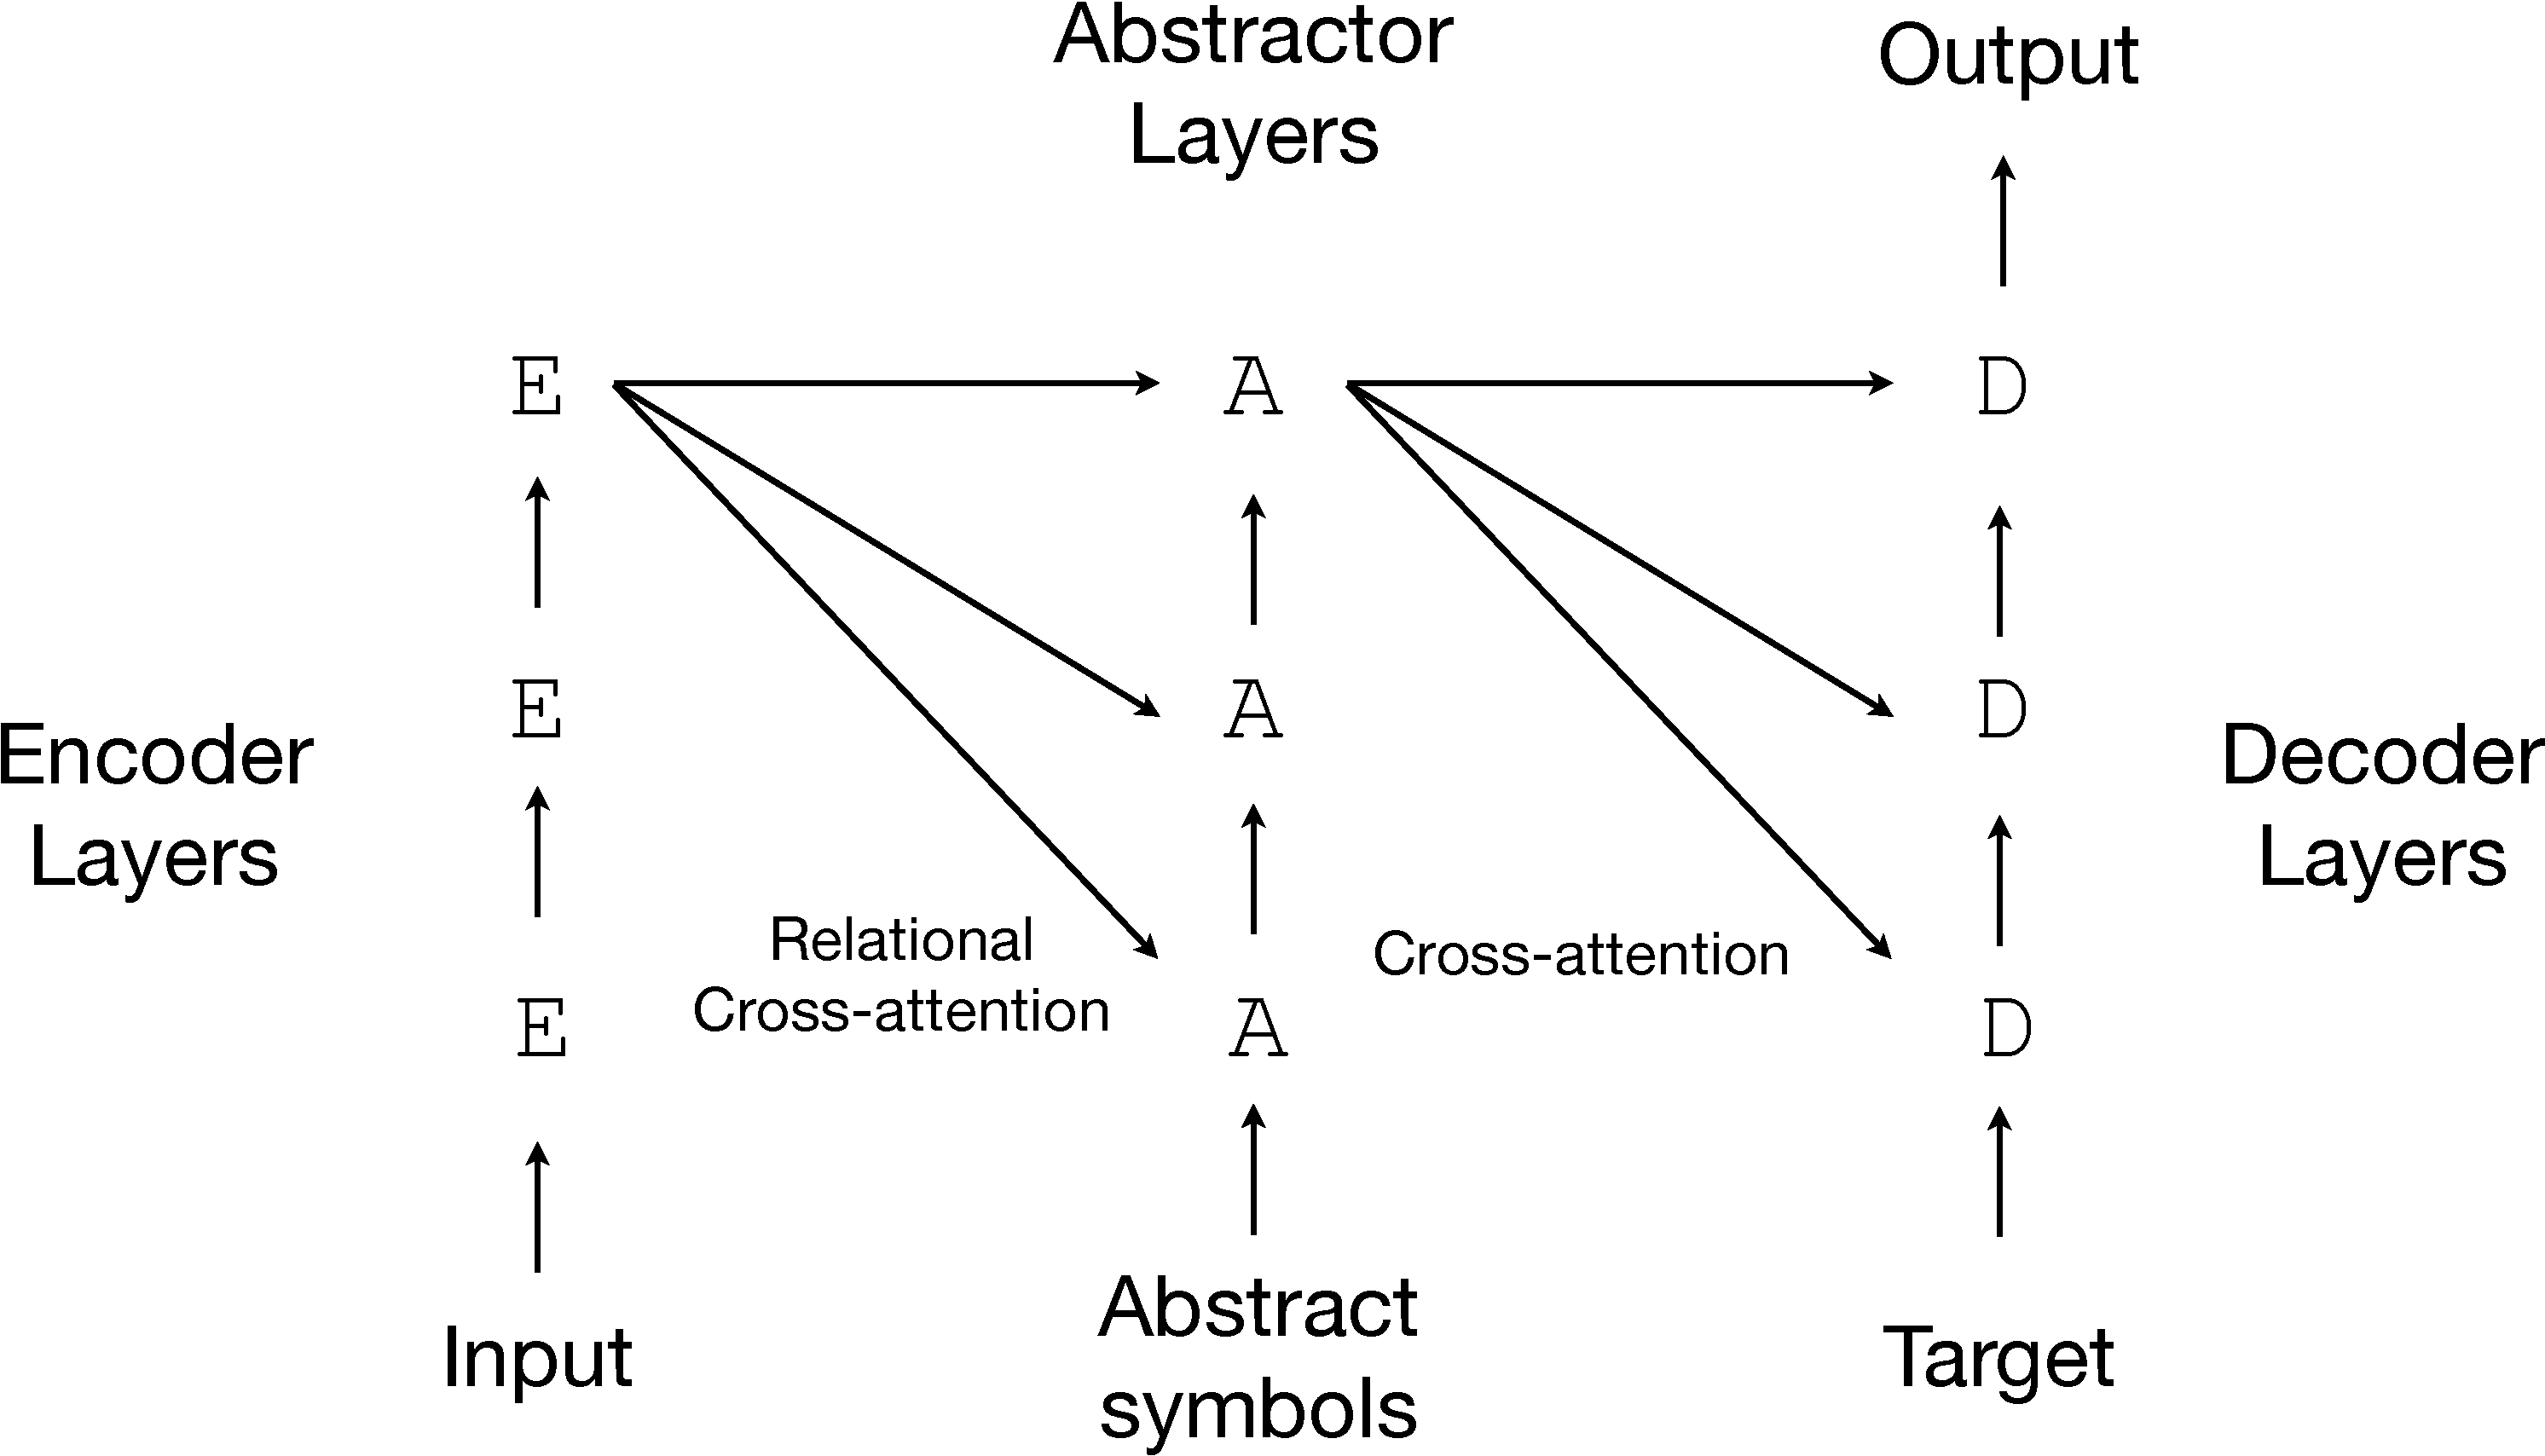
\includegraphics[width=.45\textwidth]{figures/algorithm-diagram3-crop}
        \end{tabular}
        \caption{\footnotesize Algorithmic framework integrating transformers and relational learning, 
        implementing a form of the ``relational bottleneck.''}
        \label{fig:algo}
        \end{center}
        \vskip-.15in
    \end{wrapfigure}
    %\end{figure}
The architecture has three types of states: encoder states $E$, decoder states $D$, and abstract states $A$. The encoder states are vectors that represent domain-specific information (e.g., sensory or motor), which are often successfully modeled by standard deep learning frameworks, including standard transformers. The abstract states $A$ are vectors that are learned and processed using symbolic message-passing based on the relations between the encoder states. In particular, the encoder states are separated from the abstract states by a ``relational bottleneck'' that only allows information about relations (that is, inner-products) between encoder states to influence the learning and transformation of abstract states.

This ability to integrate with transformers and process domain-specific information modeled by an Encoder gives the Abstractor framework greater flexibility compared to existing relational models like ESBN.
%If sensory information is required by the decoder, this can be passed to the decoder states $D$ by standard cross-attention mechanisms of transformers.


%
%\subsection{Example}
%\label{ssec:set}
%
%We use the game SET to illustrate relational cross-attention.
%% JDC: COULD REFERENCE WIKIPEDIA PAGE FOR SET:  https://en.wikipedia.org/wiki/Set_(card_game)
%SET is a relatively straightforward but challenging cognitive task that engages reasoning faculties in a deliberative
%, attentionally directed manner, requiring several levels of abstraction over sensory embeddings. Players are
%presented with 12 cards, each of which contains figures that vary along four dimensions (color, number, pattern, and
%shape; see Figure \ref{fig_set}a) and they must find subsets of three cards which obey a deceptively simple rule: along each dimension, all cards in a set must either have the same or unique values (e.g., in Figure \ref{fig_set}, cards with two solid blue/purple diamonds, two striped blue squiggles, and two open blue oblongs: same color, same number, different patterns, different shapes).
%
%Algorithmically, task performance can be described as follows. The visual arrangement of cards is processed into a set of encoder states $E$ by standard deep learning mechanisms. The abstractor, starting in some initial abstract state $A$, transforms the state by the evaluation of attention heads that extract relations between the cards, each head giving a relation between them in a learned attribute.
%
%\def\redcard{\colorbox{red!30}{R}\hskip.2em}
%\def\bluecard{\colorbox{blue!30}{B}\hskip.2em}
%\def\greencard{\colorbox{green!50}{G}\hskip.2em}
%\def\onecard{\fbox{\hskip1pt 1\hskip1pt}\hskip.2em}
%\def\twocard{\fbox{\hskip1pt 2\hskip1pt}\hskip.2em}
%\def\threecard{\fbox{\hskip1pt 3\hskip1pt}\hskip.2em}
%
%\begin{figure}[t]
%\begin{center}
%\begin{tabular}{ccc}
%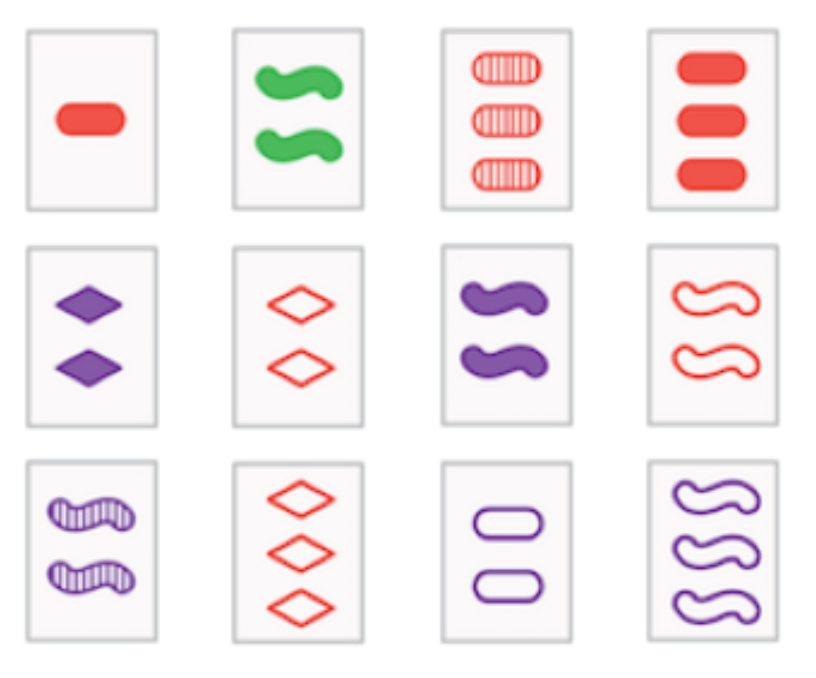
\includegraphics[width=.23\textwidth]{figures/set_example}
%& &\\[-1.15in]
%&\hskip10pt\ &\renewcommand{\arraystretch}{1.4}
%\begin{small}
%\begin{tabular}{|c|c|c|}
%%\hline
%\multicolumn{3}{c}{Attributes of encoder state $E$} \\
%\hline
%\multicolumn{1}{|c}{\redcard \redcard \redcard} & \multicolumn{1}{|c}{ \redcard\bluecard\greencard} &\multicolumn{1}{|c|}{\redcard\redcard\bluecard} \\
%\hline
%\hline
%%$\frac{1}{3}(s_1+s_2+s_3)$ & $\frac{1}{2}(s_2+s_3)$ & $s_3$ \\
%%$\frac{1}{3}(s_1+s_2+s_3)$ & $\frac{1}{2}(s_1+s_3)$ & $s_3$ \\
%%$\frac{1}{3}(s_1+s_2+s_3)$ & $\frac{1}{2}(s_1+s_2)$ & $\frac{1}{2}(s_1+s_2)$ \\
%$\frac{1}{3}(s_1+s_2+s_3)$ & $s_1$ & $\frac{1}{2}(s_1+s_2)$ \\
%$\frac{1}{3}(s_1+s_2+s_3)$ & $s_2$ & $\frac{1}{2}(s_1+s_2)$ \\
%$\frac{1}{3}(s_1+s_2+s_3)$ & $s_3$ & $s_3$ \\
%\hline
%\multicolumn{3}{c}{Transformed abstract symbol $A$}
%%\hline
%\end{tabular}
%\end{small}
%%& \\[-1.45in]
%%&&\includegraphics[width=.23\textwidth]{ppo-results/epoch_14_decision_boundaries} \vspace{-2mm} \\
%\\[10pt]
%\scriptsize (a) SET game && \scriptsize (b) Example of symbols/attention
%\end{tabular}
%\vspace{-1mm}
%\end{center}
%\caption{Illustration of mechanism used in abstractor layers with relational cross attention using the game of SET (see text for description).
%%To provide a basic working of example of abstraction in our framework,
%As an example, consider an initial abstract symbol $S = (s_1,s_2,s_3)$ for three cards, and the color attribute.
%%, for concreteness.
%Suppose a relation is learned such that  $\langle W_Q E_i, W_K E_j\rangle$ is small if cards $i$ and $j$ have different color, and is large if they are the same color.  Then relational cross-attention transforms the initial abstract symbol $S$ as shown in the above table. A multilayer perceptron can learn to discriminate between these three cases. Once learned, the symbol $A$ then can be used to represent abstract ``same/different'' relations for the sequence of inputs.}
%\label{fig_set}
%\end{figure}
%


\subsection{Configuring abstractors for different tasks}
\def\module#1{\mbox{\small\texttt{#1}}}

Abstractors can be used to approach a variety of relational learning tasks. In the case of classification
or regression, the default architecture would be
$$\module{Encoder} \rightarrow \module{Abstractor}$$
and the discriminant or regression function is computed as $f(A)$, where $A$ is the final abstract states.
For relational sequence-to-sequence tasks, the default architecture is
$$\module{Encoder} \rightarrow \module{Abstractor} \rightarrow \module{Decoder}$$

In a ``fully relational'' task, the decoder only attends to the abstractor, and therefore only uses relational information from the input. Fully relational tasks are those which can be solved using only relational information, without any information about the individual objects. An example of a fully relational task is sorting objects; we give experimental details for this example in Section~\ref{sec:experiments}.

In a ``partially-relational'' task, the relational information is crucial, but information about individual objects is also important. Here, we propose an architecture in which the decoder attends to both the abstractor and encoder modules. This can be done by either concatenating the encoder and abstractor states (i.e.: attend to $\text{concat}(E, A)$) or to iteratively cross-attend to the Encoder and Abstractor. We call this a ``sensory-connected'' Abstractor.

% JDC: IT MIGHT BE GOOD, IF POSSIBLE TO INCLUDE AN "INLINE SCHEMATIC" FOR THIS CASE AS WELL, WITH A "BYPASS" ARROW
% (RESNET STYLE) FROM ENCODER TO DECODER (THOUGH I DON'T KNOW HOW TO DO THIS IN TEX!), TO MAKE IT VISIBLY CLEAR THAT
% THE FRAMEWORK IS FLEXIBLE.
This provides an extension of general sequence-to-sequence models with transformers. In this paper, to highlight the capabilities of the framework, we focus our experiments on fully relational abstractors. However, partially relational abstractors are likely to be necessary for more realistic tasks. We hypothesize that a sensory-connected Abstractor model would yield benifits on language tasks.

We note that learning higher order relations is made possible by composing
abstractors, as in the architecture
$$\module{Encoder} \rightarrow \module{Abstractor} \rightarrow \module{Abstractor} \rightarrow \module{Decoder}.$$
Since a one-layer abstractor is able to compute a large class of functions on relations, chaining together abstractors allows the computation of relations on relations (higher-order relations). We formalize these comments in Section~\ref{sec:function_spaces}.

